\section{Trave Solaio}
\begin{pycode}[TraveSolaio]
glulam_class = 'GL28h'
kmod = 0.9
gammaM = 1.45

# Per gli SLE
k_def = 0.6
psi2_1 = 0.3
# psi0_2 =
# psi2_2 =

f_mk, f_t0k, f_t90k, f_c0k, f_c90k, f_vk, f_rk, \
E0mean, E005, E90mean, E9005, Gmean, G05, Grmean, Gr05, \
rho_k, rho_mean = glulam(glulam_class)

f_md, f_t0d, f_t90d, f_c0d, f_c90d, f_vd, f_rd = (kmod * X_k / gammaM for X_k in glulam(glulam_class)[0:7])

b = 200
h = 700
l = 7635
l_appoggio = 234 

# Sollecitazione di progetto:
Q = 34.41 #kN/m == N/mm
SLE_rara_perm = 15.6 # g1 e g2
SLE_rara_acc1 = 8.66 #carico accidentale principale
# SLE_rara_acc2 =  eventualmente aggiungerlo e de-commentare nella W_net

###########################################################
M_d = Q * l**2 / 8
V_d = Q *l / 2

W = b * h**2 / 6 #sezioni rettangolari
J = b*h**3 / 12

#Flessione:
sigma_md = M_d / W

# Sbandamento :
l_eff = 0.9*l + 2*h 

sigma_mcrit = (0.78 * b**2 * E005) / (h * l_eff) 
lambda_relm = np.sqrt(f_mk/sigma_mcrit)
if lambda_relm < 0.75:
    k_crit = 1
elif lambda_relm < 1.14:
    k_crit = 1.56 - .75*lambda_relm
else:
    k_crit = 1/(lambda_relm**2)


#Taglio    
#kcrit legno lamellare = 2.5/f_vk -> b_eff = kcr * b
b_eff = 2.5/f_vk * b
tau_d = V_d * 1.5 / (b_eff * h)

## Compressione 90 appoggio
A_ef = b* (l_appoggio+30+0) # min(30mm , a , l_appoggio, l/2) sx e dx
k_c90 = 1.75

sigma_c90_appoggio = V_d / A_ef

#Freccia
chi = 1.2
def w_inst(q): 
    w_inst_M = 5/384 * q * l**4 / (E0mean * J)
    w_inst_V = chi * 1/8 * q * l**2 / (Gmean * b * h)
    w_inst = w_inst_M + w_inst_V
    return w_inst
w_inst_perm = w_inst(SLE_rara_perm)
w_inst_acc1 = w_inst(SLE_rara_acc1)
w_netFin_perm = w_inst_perm*(1 + k_def)
w_netFin_acc1 = w_inst_acc1*(1 + k_def*psi2_1)
# w_netFin_acc2 = w_inst_acc2*(psi0_2 + k_def*psi2_2)
w_netFin_tot = w_netFin_perm + w_netFin_acc1 # + w_netFin_acc2

\end{pycode}

\begin{pysub}[TraveSolaio]
\begin{figure}[H]
    \centering
    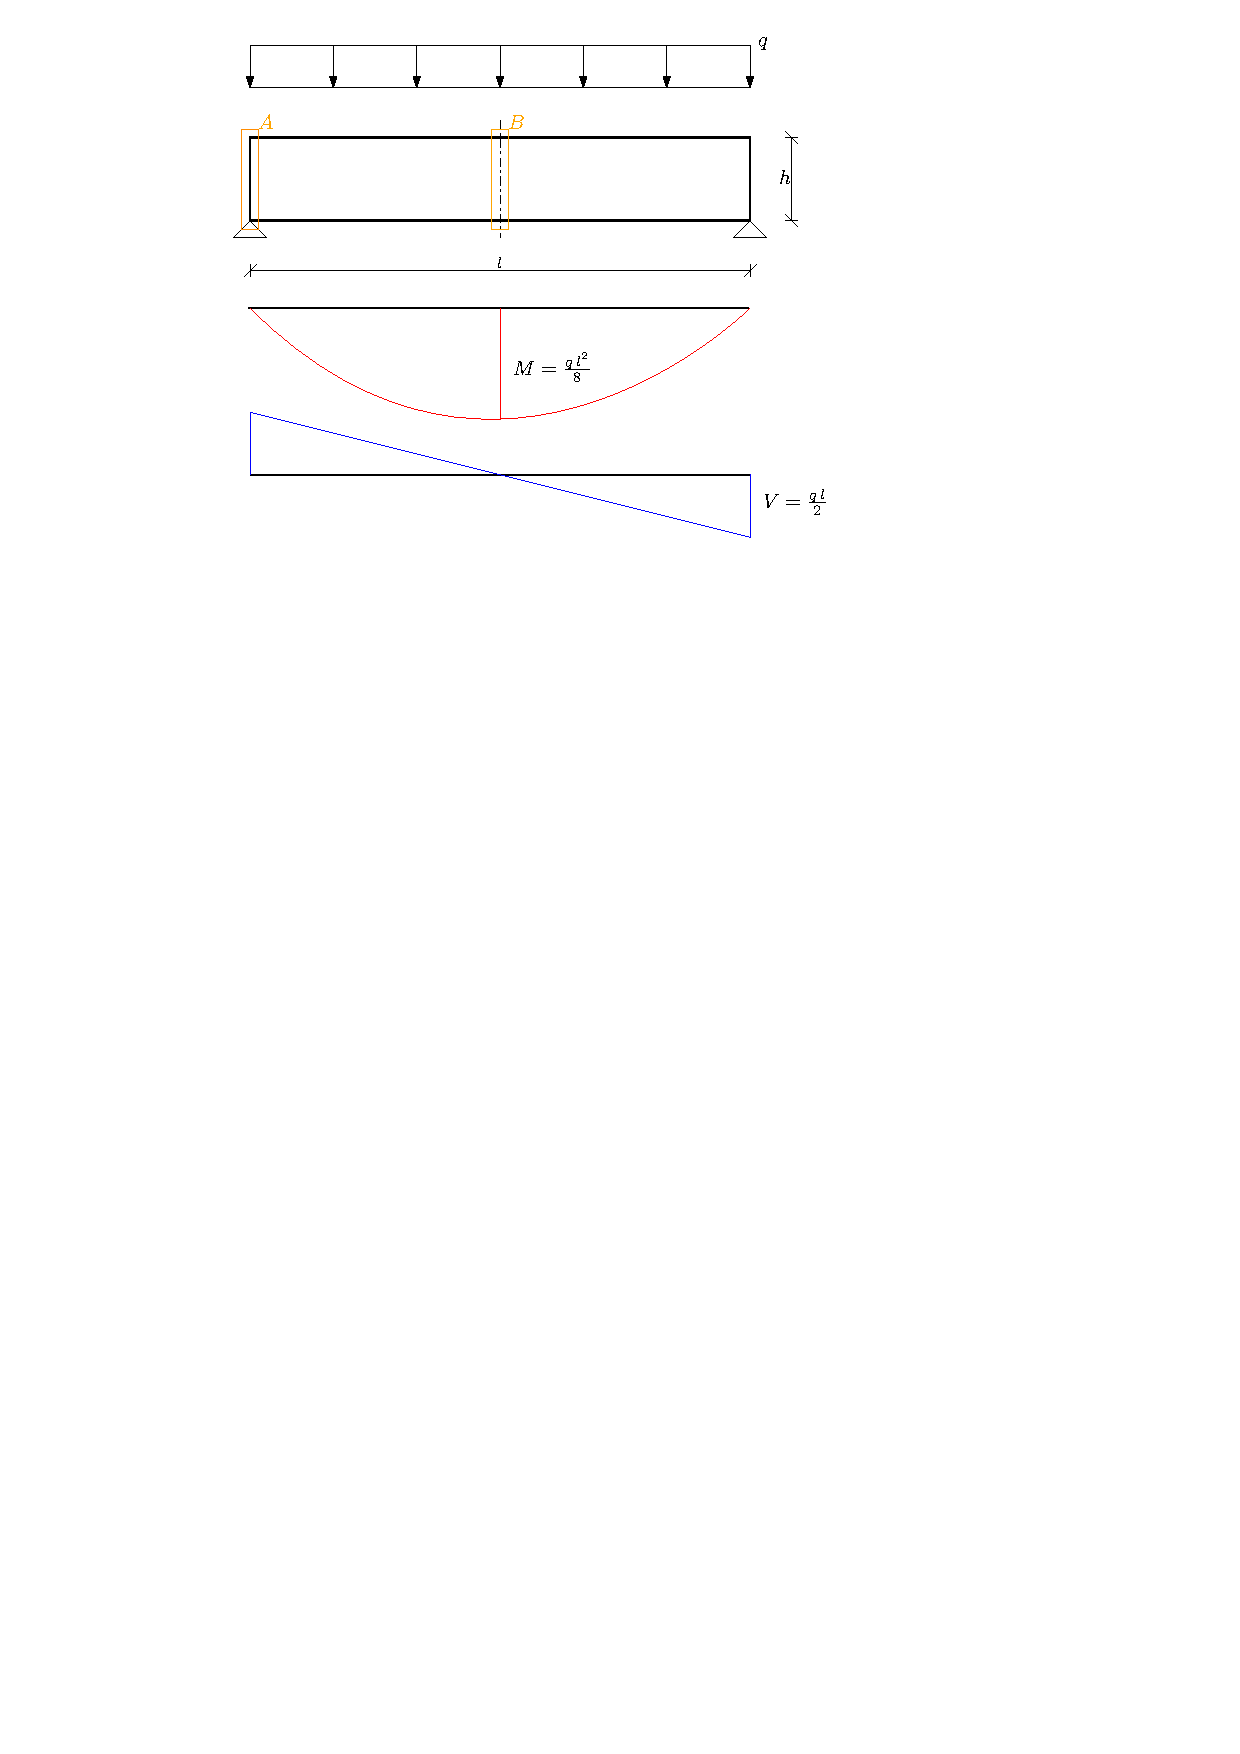
\includegraphics[]{IMG/TraveRettangolare.pdf}
    \caption{Indicazione della nomenclatura e dello schema statico adottato per la trave del solaio}
    \label{fig:TraveSolaio}
\end{figure}
\begin{table}[H]
    \centering
    \caption{Valori di progetto per la verifica della trave del solaio}
    \begin{tabular}{lS[table-format=2.2] @{\hspace{2cm}} lS[table-format=2.3]@{\hspace{2cm}} lS[table-format=5.2]}
        \toprule
		\multicolumn{6}{c}{Valori geometrici e coefficienti di esposizione o durata del carico}\\
        \midrule
		$b$      & \SI{!{b}}{\milli\metre}     & $h$        & \SI{!{h}}{\milli\metre}   & $l$           & \SI{!{l}}{\milli\metre}  \\ 
        $\gamma_M$      & \SI{!{gammaM}}{}     & $k_{mod}$        & \SI{!{kmod}}{}   & $k_{def}$ & \SI{!{k_def}}{} \\
        \midrule
        \multicolumn{6}{c}{Valori di resistenza GL28h [\si{\mega\pascal}] } \\
        \midrule
        $f_{m,k}$    & !{f_mk}   & $f_{m,d}$    & !{round(f_md,3)}  & $E_{0,mean}$ & !{E0mean} \\
        $f_{v,k}$    & !{f_vk}   & $f_{v,d}$    & !{round(f_vd,3)}  & $E_{0,05}$   & !{E005} \\
        $f_{c,90,k}$ & !{f_c90k} & $f_{c,90,d}$ & !{round(f_c90d,3)} & $G_{mean}$   & !{Gmean} \\
        $f_{t,90,k}$ & !{f_t90k} & $f_{t,90,d}$ & !{round(f_t90d,3)} &  $G_{05}$     & !{G05}\\
        \midrule
        \multicolumn{6}{c}{Valori dei carico $q$ [\si{\kilo\newton\per\metre}] } \\
        \midrule
        $SLU$    & !{round(Q,2)}   & $SLE_{rara}^{perm.}$    & !{round(SLE_rara_perm,2)}  & $SLE_{rara}^{acc. 1}$ & !{round(SLE_rara_acc1,2)} \\
        \bottomrule
    \end{tabular}
\end{table} 
\begin{table}[H]
    \centering
    \caption{Azioni di progetto SLU nei punti di sezione indicati in figura per la trave del solaio}
    \begin{tabular}{c  S[table-format=4.1] S[table-format=4.3] S[table-format=3.3]}
        \toprule
		%\multicolumn{4}{c}{Azioni di progetto nei punti di sezione}\\
        Sezione & \multicolumn{1}{c}{$x$ [\si{\milli\metre}]} & \multicolumn{1}{c}{$M_d$ [\si{\kilo\newton\metre}]}& \multicolumn{1}{c}{$V_d$ [\si{\kilo\newton}]} \\
        \midrule
        A & 0. 0               & 0.0                      & !{round(V_d/10**3,3)}   \\
        B & !{round(l/2,1)}    & !{round(M_d/10**6,3)}    & 0.0						\\
        \bottomrule
    \end{tabular}
\end{table} 
Si riportano ora le verifiche svolte calcolate in base al capitolo 6 dell'Eurocodice 5 (UNI EN 1995-1-1), salvo diversamente specificato.
\subsection{Flessione}
\begin{equation} 
    \sigma_{m,d} \leq f_{m,d} = \SI{!{round(f_md,3)}}{\mega\pascal}
\end{equation}

La sollecitazione massima la si ha in mezzeria, pertanto è pari, avendo sezione rettangolare, a:
\[
\sigma_{m,d} 
= \frac{M_d}{W} 
= \frac{M_d}{\dfrac {b \cdot h^2}{6}} 
= \frac{\SI{!{round(M_d/10**6,3)}e6}{\newton\milli\metre}} {\dfrac {!{b} \cdot !{h}^2}{6} \si{\milli\metre\tothe{3}}} 
= \SI{!{round(sigma_md,3)}}{\mega\pascal} 
\]


\subsection{Stabilità flesso-torsionale}
Si deve avere
\begin{equation}
     \sigma_{m,d} \leq k_{crit} \cdot f_{m,d} 
\end{equation}
dove 
\begin{equation}
    k_{crit} =
    \begin{cases}
        1 & \text{se \quad $ \lambda_{rel,m} \leq 0.75$} \\
        1.56 - 0.75 \cdot \lambda_{rel,m} & \text{se \quad $0.75 \leq \lambda_{rel,m} \leq 1.4$} \\
        \dfrac{1}{\lambda_{rel,m}^2} & \text{se \quad $\lambda_{rel,m} \geq 1.4$}
    \end{cases}
    \quad =  !{round(k_crit,3)}
\end{equation}
in cui 
\[
\begin{split}
    \lambda_{rel,m} 
    &= \sqrt{  \frac{f_{m,k}}     {\sigma_{m,crit}}          } 
    = \sqrt{  \frac{!{f_mk}}     {!{round(sigma_mcrit,1)}}  } 
    = !{round(lambda_relm,3)} \\
    \sigma_{m,crit} 
    &= \dfrac{0.78}{l_{eff}} \dfrac{b^2}{h} E_{0.05}
    = \dfrac{0.78}{!{round(l_eff,1)}} \dfrac{!{b}^2}{!{h}} !{E005}
    = \SI{!{round(sigma_mcrit,1)}}{\mega\pascal} \\
    l_{eff}  
    &= 0.9 \, l + 2 \, h
    = 0.9 \cdot !{round(l,1)} + 2 \cdot !{h}
    = \SI{!{round(l_eff,1)}}{\milli\metre}
\end{split}
\]
essendo il carico nel bordo compresso dell'elemento.

Quindi la verifica diventa
\[
    \SI{!{round(sigma_md,3)}}{\mega\pascal} <  !{round(k_crit,3)} \cdot \SI{!{round(f_md,3)}}{\mega\pascal} = \SI{!{round(k_crit * f_md,3)}}{\mega\pascal}
\]
risultando pertanto soddisfatta.

\subsection{Taglio}
Si deve avere
\begin{equation}
    \tau_d \leq f_{v,d}   
\end{equation}
La sollecitazione massima che si ha agli appoggi vale
\[
\tau_d 
= 1.5 \frac{V_d}{b_{eff} \cdot h} 
= \frac{\SI{!{round(V_d/10**3,3)}e3}{\newton}} {!{round(b_eff,1)} \cdot !{h} \si{\milli\metre\tothe{2}}} 
= \SI{!{round(tau_d,3)}}{\mega\pascal} 
\]
in cui da normativa NTC (C.4.4.8.1.9) per il legno lamellare 
\[
    b_{eff} 
    = k_{cr} \cdot b 
    = \dfrac{2.5}{f_{v,k}} \cdot b 
    = \dfrac{2.5}{!{f_vk}} \cdot !{b}
    = \SI{!{round(b_eff,1)}}{\milli\metre}
\]
Essendo $\SI{!{round(tau_d,3)}}{\mega\pascal} < \SI{!{round(f_vd,3)}}{\mega\pascal}$ la verifica è soddisfatta.

\subsection{Compressione perpendicolare appoggio}
Si deve avere 
\begin{equation}
    \sigma_{c,90,d} \leq k_{c,90} \cdot f_{c,90,d}
\end{equation}
in cui $k_{c,90}$ vale $!{k_c90}$ per il legno lamellare e $f_{c,90,d}$ è pari a \SI{!{round(f_c90d,3)}}{\mega\pascal}.

La tensione all'appoggio si calcola come
\[
    \sigma_{c,90,d} = \frac{V_d}{A_{ef}} = \frac{\SI{!{round(V_d/10**3,3)}e3}{\newton}}{\SI{!{round(A_ef,1)}}{\milli\metre\squared}} = \SI{!{round(sigma_c90_appoggio,3)}}{\mega\pascal}
\]
in cui $A_{ef}$ consiste nell'area di contatto efficace $b \cdot l_{ef}$, calcolata aumentando la lunghezza di appoggio della scarpa mettallica (che vale \SI{!{l_appoggio}}{\milli\metre}) di \SI{30}{\milli\metre} in un solo lato.

Si ha quindi
\[
    \SI{!{round(sigma_c90_appoggio,3)}}{\mega\pascal} <  !{round(k_c90,3)} \cdot \SI{!{round(f_c90d,3)}}{\mega\pascal} = \SI{!{round(k_c90 * f_c90d,3)}}{\mega\pascal}
\]

\subsection{Freccia}
La freccia dovuta al contributo del momento flettente e del taglio, nel caso di semplice appoggio vale
\begin{equation}
    w(q) = \dfrac{5}{384} \frac{q \cdot l^4}{E_{0,mean} \cdot J} + \chi \dfrac{1}{8} \frac{q \cdot l^2}{G_{mean} \cdot b \cdot h}
\end{equation}
che, per un carico unitario e per una sezione rettangolare, assume il valore di riferimento
\begin{equation}
    w(q = \SI{1}{\kilo\newton\per\metre}) 
    = \dfrac{5}{384} \frac{1 \cdot !{l}^4}{!{E0mean} \cdot \SI{!{round(J/10**6,3)}e6}{}} + !{chi} \dfrac{1}{8} \frac{1 \cdot !{l}^2}{!{Gmean} \cdot !{b} \cdot !{h}} 
    = \SI{!{round(w_inst(1),3)}}{\milli\metre}
\end{equation}

Le deformazioni istantanee per i carichi agli SLE con combinazione rara valgono:
\begin{align}
    w_{inst,G}
    &= w(q = \SI{!{round(SLE_rara_perm,2)}}{\kilo\newton\per\metre}) 
    = \SI{!{round(w_inst_perm,2)}}{\milli\metre}  \\
    %
    w_{inst,Q1}
    &= w(q = \SI{!{round(SLE_rara_acc1,2)}}{\kilo\newton\per\metre}) 
    = \SI{!{round(w_inst_acc1,2)}}{\milli\metre}
    \quad\Longrightarrow\quad
    l/w_{inst,Q1} = \SI{!{round(l/w_inst_acc1,1)}} \,>\, 300\\
    %
    w_{inst,TOT}
    &= w_{inst,G} + w_{inst,Q1}
    = \SI{!{round(w_inst_perm + w_inst_acc1,2)}}{\milli\metre}
\end{align} %

Con $k_{def} = !{k_def}, \psi_{21} = !{psi2_1}$, in assenza di controfreccia iniziale e nelle ipotesi che gli elementi abbiano lo stesso comportamento viscoelastico, le deformazioni finali per i carichi agli SLE con combinazione rara assumono la forma semplificata:
\begin{align}
    w_{fin,G}
    &= w_{inst,G} \cdot (1 + k_{def})
    = \SI{!{round(w_netFin_perm,2)}}{\milli\metre}  \\
    %
    w_{fin,Q1}
    &= w_{inst,Q1} \cdot (1 + \psi_{21} \, k_{def})
    = \SI{!{round(w_netFin_acc1,2)}}{\milli\metre} \\
    %
    w_{fin,TOT}
    &= w_{fin,G} + w_{fin,Q1}
    = \SI{!{round(w_netFin_tot,2)}}{\milli\metre}
    \quad\Longrightarrow\quad
    l/w_{fin,TOT} = \SI{!{round(l/w_netFin_tot,1)}} \,>\, 200
\end{align} %

\end{pysub}
